\documentclass[11pt,a4paper]{article}
\usepackage[utf8]{inputenc}
\usepackage[spanish]{babel}
\usepackage{amsmath}
\usepackage{array}
\usepackage{multirow}
\usepackage{float}
\usepackage{amsfonts}
\usepackage{amssymb}
\author{Walter Gonzalez\\ \\
\small{Facultad de Ciencias Económicas, Universidad Nacional de Córdoba}\\
\small{\texttt{walterignaciogonzalez@gmail.com}}
}
\title{Brecha cambiaria en Argentina: La relación entre los múltiples tipos de cambio}
\date{Octubre 2020}
\usepackage[left=2.5cm,right=1.5cm,top=2.5cm,bottom=2.5cm]{geometry}
\usepackage{tcolorbox}
\setcounter{MaxMatrixCols}{20}
\usepackage{graphicx}
\usepackage{float}




\begin{document}
\maketitle
\begin{abstract}
En Argentina durante el segundo semestre de 2019, un conjunto de restricciones cambiarias originaron tipos de cambios múltiples, que si bien existían antes de ellos no eran precios de referencia generalizados. Entre ellos están (en relación al peso) el oficial, el solidario, el blue y el MEP. En este artículo se analizan las interdependencias entre ellos mediante modelos VECM. En concordancia con otros trabajos se encuentra que cuando la brecha entre el oficial y el blue es mayor que el valor de largo plazo, el desequilibrio se resuelve con un aumento del valor del tipo de cambio oficial. Además se encuentra que el dolar blue depende del dolar MEP y no a la inversa. Por lo que se podría justificar una política de corto plazo, que mantenga la brecha cercana a los valores de largo plazo a fin de que al momento de levantar las restricciones la devaluación sea relativamente menor
\end{abstract}

\clearpage


\tableofcontents
\clearpage

\section{Introducción}
En las economías en desarrollo y particularmente en las latinoamericanas suele repetirse con cierta regularidad crisis cambiarias. Estos procesos son normalmente originados en financiación del déficit fiscal con deuda externa principalmente, donde los flujos de capital suelen ser detenidos abruptamente en lo que en Dornbusch (1995) y Calvo (1998) se dió a conocer como ``Sudden Stop''. Generalmente estas son crisis de liquidez y no de solvencia, donde a veces puede darse un default de la deuda soberana, pero siempre se ve aparejado una crisis cambiaria debido a la falta de divisas. Ante este último problema, los gobiernos suelen presentar sistemas de control de cambios para evitar o retrasar una devaluación en orden no desestabilizar todavía mas el orden macroeconómico. Si bien el origen de estos sistemas es transitorio, en Argentina estos suelen prolongarse varios años, lo que incentiva a los agentes a valorar de una manera especial las monedas externas. Particularmente al dólar. Es entonces cuando las restricciones generan diversos mercados donde se comercializan estas divisas entre privados, entre los cuales se encuentra el dolar blue, que es el nombre que se le da al que se compra y vende ilegalmente en el mercado negro. La brecha que existe entre el oficial y el blue, es de gran importancia ya que si es muy grande aumentan los incentivos a comprar en el primero y vender en el segundo, desplazando la oferta de divisas al mercado paralelo y aumentando la demanda en el legal. Esto genera un ``efecto goteo'' (Dornbusch, 1986) que reduce aún mas las reservas internacionales por lo que las autoridades deben endurecer los controles o permitir finalmente la devaluación.

Este proceso a sido teorizado y medido empíricamente en diversos momentos y para muchos países, y ciertamente con foco en Argentina también. Pero todavía no se tienen trabajos que lo cuantifiquen después del año 2015. Además todos los trabajos suelen explorar la relación entre el dolar oficial y el blue, dejando de lado el resto de mercados cambiarios como el MEP o el contado con liquidación. Por lo que este es el primer artículo que explora las interdependencias entre todos los mercados. La motivación de esta búsqueda es que la historia ha demostrado que los controles de cambios suelen provocar una suerte de ``bola de nieve'', ya que cuando son eliminados la devaluación es casi del mismo valor que la brecha cambiaria, por lo que muchos gobiernos han intentado disminuirla con rústicos instrumentos como la coerción. Si pudiera mantenerse contenido el valor del dolar blue aprovechando esas interdependencias, podría crearse la posibilidad de utilizar un nuevo instrumento que haga menos costoso el fin de los controles.

Luego de esta sección introductoria el trabajo seguirá con una breve contextualización de los mercados cambiarios en el país; cuales son, las conclusiones que artículos anteriores han encontrado y cual ha sido su evolución en los últimos años. Después se describirá el modelo econométrico que será utilizado y los resultados del mismo. Por último, se resumirán las conclusiones. En el anexo se podrán observar los test que corroboran el cumplimiento de los supuestos del modelo.


  
\section{Tipo de cambio en Argentina}

\subsection{Controles cambiarios y tipos de cambios múltiples}
Según Bagwhati (1979) hay dos tipos de controles cambiarios, aquellos que son una restricción en la cantidad de divisas que pueden ser adquiridas y otros que representan una regulación sobre el precio al que puede adquirirse. En la última década en Argentina se han utilizado ambas, y generalmente, al mismo tiempo. Cronológicamente puede dividirse según los siguientes hitos:
\begin{itemize}
\item Las primeras restricciones fueron autorizadas el 28/11/2011. Se decidió que las personas o empresas que quieran adquirir dolares, deberían tener una autorización especial de AFIP.
\item El 9/02/2012 se reguló que empresas que deban girar dinero al exterior ya sea por ganancias, importaciones o deuda, debían tener una autorización especial la cual era entregada discrecionalmente y podía demorarse varios meses 
\item El 15/06/2012 se eliminó la posibilidad de comprar dólares para ahorro y sólo se podían comprar en caso de viajes
\item El 30/08/2012 se estableció una retención del $15 \% $ sobre consumos en el exterior con tarjeta tomado como un anticipo de otros impuestos como Bienes Personales o Ganancia. En 2013 esta alícuota aumentó a $20 \% $ primero y $35 \% $ después
\item El 16/12/2015 se liberó el mercado cambiario.
\item El 01/09/2019 se dispuso un límite de 10000 dólares mensuales por persona. Al final del mes siguiente, este límite bajó a 200
\item El 21/12/2019 se estableció un impuesto del $30 \% $ para la compra de divisas. 
\item El 15/09/2020 se estableció una retención similar a la de 2012 como anticipo de otros impuestos, con una porcentaje del $35 \% $ del valor oficial
\end{itemize}
Como se mencionó anteriormente, estas restricciones dieron origen a varios mercados donde los individuos pueden acceder a la divisa externa.

El primero de estos es el dolar oficial. En los momentos en los cuales no existen regulaciones, es el único precio de referencia. Pero cuando si existen, es prácticamente inaccesible para los individuos\footnote{En las regulaciones de mediados de 2020 solo los hijos de desaparecidos puede acceder al mismo} y solo algunos sectores mayoristas pueden acceder a su compra. Aún así, la mayoría de las actividades de exportación son liquidadas a este precio, lo cual obviamente las desalienta en el mediano plazo.

Luego está el dolar solidario, que también puede ser llamado dolar ahorro o dolar turismo en función de si existen diversos aranceles para cada uno de estas actividades. Para el período en cuestión es un $30 \% $ mayor al oficial primero y un $65 \%  $ mayor a partir de septiembre de 2020

El dolar blue es el dolar ilegal que se compra y vende en el mercado negro, particularmente formado por casas de cambio y financieras. En la práctica son muy visibles en las zonas céntricas de las ciudades.

El contado con liqui es el tipo de cambio que surge de una operación financiera en la que se compra una acción que cotiza en el mercado local en moneda doméstica y se vende en el mercado externo en dólares. La diferencia de las cotizaciones en ambos mercados sobre (relativamente) el mismo activo es el que determina su valor. Esta operación es legal y no tiene cupo.

Por último, el dolar MEP es similar al contado con liquidación, pero se opera únicamente en el mercado local por lo que no se necesita tener una cuenta en el exterior. Se compra un bono determinado denominado en pesos y se cambia por el mismo bono denominado en dolares (como es el mismo bono en cuanto a cronograma de pagos, se asegura que la única diferencia que existe entre ambos es cambiaria) el cual se vende para adquirir la divisa. Es legal y no tiene cupo, pero puede estar regulado por el ``parking''; un período durante el que se tiene que mantener el bono en pesos antes de ser cambiado que puede durar entre 3 y 5 días hábiles. 



\subsection{Revisión bibliográfica}
La literatura existente sobre los controles de cambio es amplia y variada. Si bien existió cierto auge en la etapa de la economía mundial en salida del patrón oro, hasta la década del 70 no se contaba con modelos matemáticos precisos que pudieran teorizar estos comportamientos ni la econometría suficiente para medirlos. Uno de los primeros fue el que se encuentra en Barro (1977) y modificado por Hoffman et al (1984) que permite testear el impacto de shocks anticipados y no anticipados, a partir de una ecuación que permite a los agentes predecir los movimientos del tipo de cambio. Aún así, el modelo mas presente en los trabajos incluso de la actualidad es el propuesto en Dornbusch et al. (1983). Este modelos postula dos comportamientos, por un lado la oferta de dolares en el mercado negro es predeterminada por lo que la brecha con el dolar oficial ajusta para equilibrar el primer mercado y luego la brecha cambiaria determina el ritmo al cual varía el el stock de activos externos del país. Sobre este modelo trabajaron Kamin (1993), para analizar programas de estabilización para América Latina y Diamandis et al. (2005) que agregó un componente de expectativas sobre cotizaciones futuras de la divisa, para luego medirlo. 

En cuento a los trabajos netamente empíricos hay dos grandes grupos. Aquellos que han usado la metodología de datos de panel y los que han utilizado estimaciones de series de tiempo. Dentro de los primeros los trabajos realizados por Easterly tienen gran importancia. Dicho autor empleó regresiones de corte transversal en 1993 para mas de 50 países entre 1970 y 1985, luego utilizó un panel para 16 países de América Latina (Easterly, 2001), y finalmente presentó un panel para 82 países entre 1960 y 2000 en Easterly (2004). El principal objetivo de estos trabajos era medir el impacto de la brecha en el crecimiento, en los cuales se encontró que ambos están negativamente relacionados pero con una relativamente baja importancia. Mas cercano en el tiempo, en Libman (2008) se estima un panel para 7 países latinoamericanos entre 1950 y el 2000, en el cual se prioriza el análisis del comportamiento de la brecha en sí misma. Se encuentra que existen valores de largo plazo para la brecha cambiaria, y que desviaciones de estos valores se corrigen con devaluaciones del tipo de cambio oficial y no con variaciones del tipo de cambio negro.

En cuanto al segundo grupo, existía un problema habitual en la disciplina, en la cual los trabajos no tenían en cuenta la cointegración entre variables. Por lo cual la validez de los supuestos utilizados está en duda al no poder decidir si las combinaciones lineales entre series son estacionarias o no. Entre estos están Malone y ter Horst (2010) , Fishelson (1988) , Phylaktis (1992) y Shachmurove (1999). Las conclusiones de estos trabajos confirman la presencia de autocorrelación entre la brecha y sus valores rezagados. Por lo que la metodología de series de tiempo actual resulta muy apropiada para analizar estos procesos, particularmente los modelos VEC.

Es usada en Lemma (2004) \footnote{Se observa, una relación inversa entre el valor del dolar blue y las reservas disponibles en el país y una correlación positiva con la base monetaria, la depreciación del tipo de cambio oficial y los impuestos a la exportación} donde se prioriza encontrar los principales determinantes del precio del dolar informal para Etiopía. Este trabajo fue adaptado por Gimenez Rixrath (2015) para el caso argentino encontrando que el dólar blue está positivamente correlacionado con el nivel de reservas del Banco Central y las trabas a la exportación e inversamente relacionado con la base monetaria, las trabas a las importaciones y el MERVAL (principal índice del mercado bursátil argentino). Tomando estos trabajos, en Pineda Molina (2016) se analizan los determinantes del dolar MEP, encontrando una relación positiva entre este y el oficial para el período 2013-2015. Sin embargo, no se encontraron trabajos que analicen la relación entre el blue y el MEP, por lo cual este será uno de los aportes que se realizará en este artículo. 

\subsection{Contextualización del período}
El tipo de cambio en Argentina es una variable históricamente volátil y que tiende al alza. Desde la liberación del mercado cambiario en 2015 existe una flotación controlada del precio del dólar, donde el BCRA\footnote{Banco Central de la República Argentina} interviene con compras y ventas para regular las fuerzas de mercado. Durante estos años, el gobierno decidió financiar el déficit fiscal con endeudamiento externo. Las divisas que entraban eran por un lado atesoradas por el banco central para lo cual se emitía para que el tesoro realice sus pagos y por otro eran ofertadas en el mercado oficial. Durante este tiempo, el ingreso constante de divisas empezó a disminuir el tipo de cambio real, ya que el nominal estaba relativamente fijo (por la oferta del tesoro) y la inflación anual rondó entre el $20 \% - 55 \%$. El BCRA para esterilizar su propia emisión, ya que presentaba un esquema de inflation targeting, emitió letras especiales llamadas LEBACS que pagaban un alta tasa ya que debían estar por encima de la inflación para anclar expectativas. Esto incentivó aún mas el ingreso de capitales especulativos que querían aprovechar estas altas tasas en un contexto mundial donde el interés en el resto del mundo era relativamente bajo, y que el tipo de cambio estaba estable. Por supuesto esta inversión requiere volver al activo dolar antes de una devaluación que licue el rendimiento. Esto se vio en 2018 donde cierta restricción de capitales externos y poca credibilidad en el plan económico del gobierno hicieron que la oferta de divisas disminuya y al aumentar el precio del dolar, los inversionistas de riesgo supusieron que era el momento de liquidar sus inversiones en el país, por lo que aumentó la demanda de la divisa. Si bien al principio no hubo problemas ya que el BCRA pudo abastecer esta demanda ya que había acumulado reservas, pronto empezaron a escasear por lo que subió aún mas la tasa de LEBACS para incentivar el roll over. Este stock de deuda doméstica, igualó a la base monetaria en 2019, por lo cual cada vencimiento de intereses significaba un aumento de la emisión que ya directamente iba al dolar, porque nadie creía que se podría evitar una gran devaluación. El tipo de cambio ya había aumentado, se había firmado un tratado de ayuda financiera con el FMI y la presiones devaluatorias continuaban, por lo que se decidió empezar con los controles cambiaros. Tímidos al principios y estrictos a partir de octubre del 2019. Dos meses después se decidió establecer el ``impuesto país'', un arancel a la compra de divisas descripto en la subsección anterior. A partir de allí empezaron a calcularse los tipos de cambios múltiples ya que antes del mismo, y el conjunto de restricciones, el dolar de referencia era el oficial. 

\begin{figure}[H]
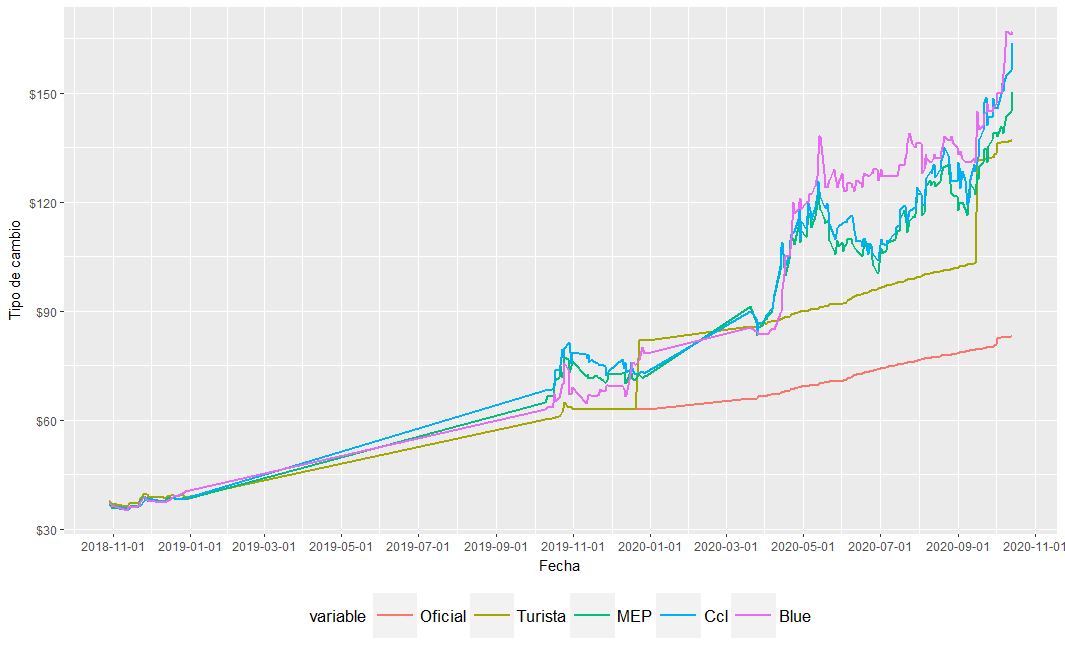
\includegraphics[scale=0.45]{1}
\centering
\caption{Evolución de los tipo de cambios}
\end{figure} 

En esta figura se observa como la cotización de los tipos de cambio durante fines de 2018 y hasta octubre del 2019 es bastante suave en términos de sus variaciones. Pero a partir del comienzo de las restricciones esto no ocurre 

\begin{figure}[H]
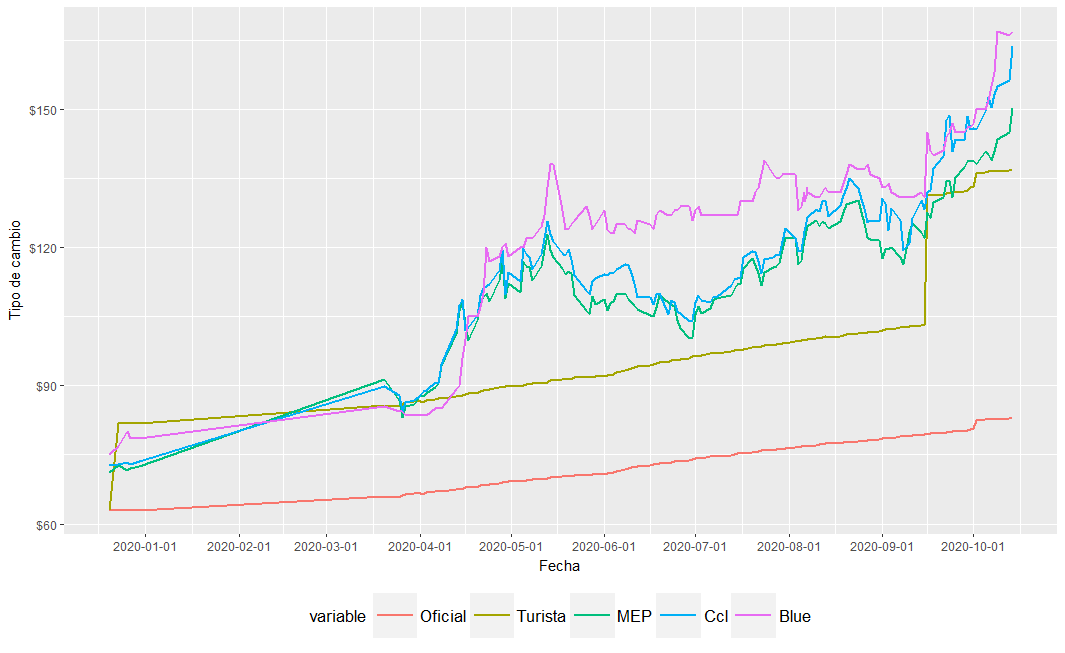
\includegraphics[scale=0.45]{2}
\centering
\caption{Evolución de los tipo de cambios (desde impuesto país hasta 30/9)}
\end{figure}

Desde el impuesto país, se ve como el dolar oficial continua una trayectoria sin grandes picos y apenas creciente. Mientras que todos los otros tipos de cambio, sufren grandes variaciones y su crecimiento es mucho mayor. Además es importante notar que estas variaciones parecen estar correlacionadas, lo que es importante para suponer que existe cointegración entre las variables. 
\begin{figure}[H]
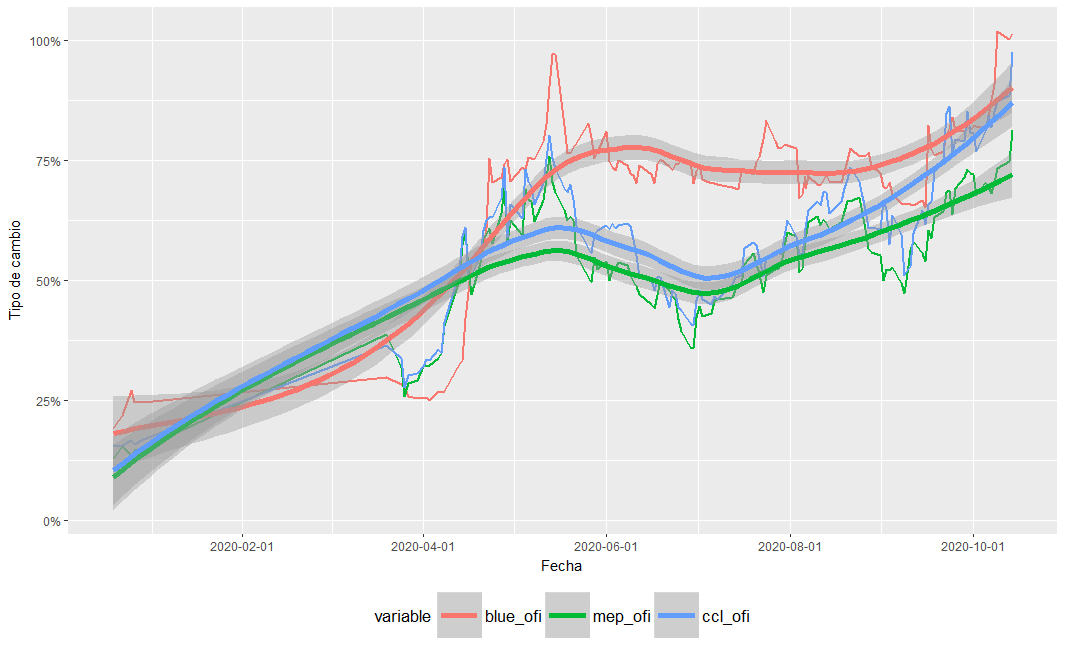
\includegraphics[scale=0.45]{3}
\centering
\caption{Evolución de las brechas sobre el dolar oficial desde el impuesto país}
\end{figure} 

\begin{figure}[H]
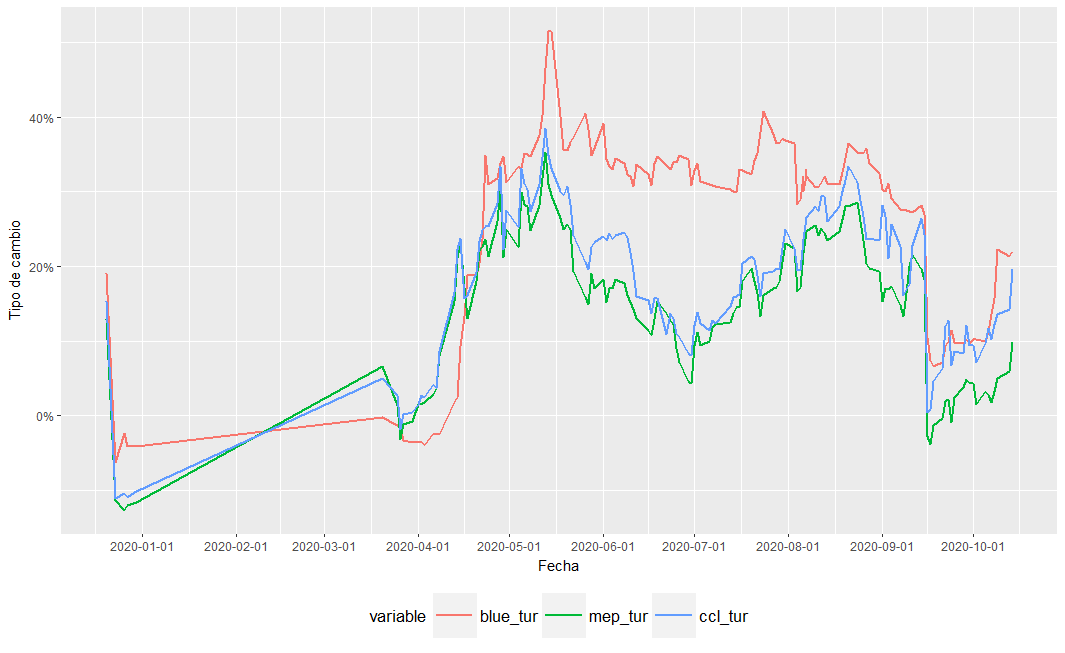
\includegraphics[scale=0.45]{4}
\centering
\caption{Evolución de las brechas sobre el dolar ahorro/turístico desde el impuesto país}
\end{figure} 

Esta cointegración es aún mas evidente cuando se observan las brechas cambiarias. El dolar oficial mide la brecha típica, pero no es representativa de los cambios ya que existen dos períodos con distintos aranceles para la compra de divisas oficiales, y además nadie puede conseguirla a este precio. Por lo que solo sirve de referencia para las exportaciones. El proceso de comprar dolares oficiales y venderlos en el mercado negro, tiene como referencia la brecha con respecto al dolar ahorro. Por lo que será este el utilizado en las estimaciones, ya que el dolar oficial no está cointegrado al resto de las variables.

\section{El modelo}

Como se mencionó anteriormente, muchos trabajos de relativa antigüedad realizaban estimaciones de serie de tiempo únicamente con Mínimos Cuadrados Ordinarios (MCO) o modelos de vectores autorregresivos (VAR). Ambas requieren que las variables sean estacionarias, si bien la primera lo requiere en niveles y los VAR en diferencias. Esto significa que la media y todas las autocovarianzas de la serie son finitas y, sobretodo, no cambian con el tiempo.
En las series económicas típicas, es muy común encontrar que son estacionarias en primeras o a lo sumo segundas diferencias. Estos procesos son conocidos como integrados de orden $d$, $1-\mathrm{I}(d)$ siendo $d$ la cantidad de veces que hay que diferenciar la serie para que sea estacionaria. Pero existe un potencial peligro cuando se realizan estimaciones entre varias series, que es la cointegración. Esto significa que dos variables comparten cierta tendencia en el tiempo, por lo que existe una relación entre ellas en el largo plazo que corrige las desviaciones del corto plazo. Modelar un VAR cuando existe cointegración, revela un sesgo en las estimaciones al no tener en cuenta esta ``tracción'' del largo plazo, el cual es justamente el que se corrige en un VECM (Vector error correction model).

Siguiendo a Enders (2008) una relación de cointegración entre dos variables se evidencia cuando se cumple que para las variables $y_t$ y $z_t$:
$$
\beta_1 y_t + \beta_2 z_t = 0
$$

Un ejemplo de esto puede ser observado suponiendo que:
$$
\begin{aligned}
y_{t} &=\mu_{t}+\varepsilon_{y t} \\
z_{t} &=\mu_{t}+\varepsilon_{z t} \\
\mu_{t} &=\mu_{t-1}+\varepsilon_{t}
\end{aligned}
$$

Por construcción $\mu_t $ es un random walk, $y_{t} , z_{t}$ son $I(1)$ y  $\varepsilon , \varepsilon_{y t}, \varepsilon_{z t} $ son procesos estacionarios. Entonces, utilizando un vector de cointegración $\beta(1,-1) $:
$$
y_{t}-z_{t}=\left(\mu_{t}+\varepsilon_{y t}\right)-\left(\mu_{t}+\varepsilon_{z t}\right)=\varepsilon_{y t}-\varepsilon_{z t}
$$
En donde se obtiene un proceso estacionario a partir de la suma de dos variables que no lo son. Enders (2008) en las páginas 355-360, demuestra que la estimación de un VAR típico es inapropiada por no tomar el efecto de la cointegración a largo plazo. Por esto se debe realizar la estimación de un VECM que para el caso de $n $ variables $x_{t}=\left(x_{1 t}, x_{2 t}, \ldots, x_{n t}\right)^{\prime}$ consiste en la estimación de las siguientes ecuaciones:

$$
\Delta x_{t}=\pi_{0}+\pi x_{t-1}+\pi_{1} \Delta x_{t-1}+\pi_{2} \Delta x_{t-2}+\cdots+\pi_{p} \Delta x_{t-p}+\varepsilon_{t}
$$

Donde 
\begin{itemize}
\item $\pi_{0}$ es el vector de constantes
\item $pi$ es una matriz que contiene la velocidad de ajuste al largo plazo entre las variables, donde al menos uno de sus elementos debe ser diferente a cero, ya que si no lo fuera, la estimación sería idéntica a la de un VAR común. Si todos los elementos de la fila $k$ son iguales a cero, esto significa que la variable $x_k$ es ``débilmente exógena''. Esto significa que, en presencia de cointegración, esta variable no es afectada por las variaciones respecto al los niveles de estabilidad de largo plazo, por lo que todo el ajuste desde el corto al largo plazo es realizado por otras variables 
\item $\pi_{i}$ contiene los coeficientes típicos que relacionan las variables $n $ entre sí en el corto plazo, con una $p$ cantidad de lags 
\item $\varepsilon_{t} $ son los errores de predicción del modelo, y deberían simular un proceso de ruido blanco
\end{itemize}

Esta ecuación puede estimarse directamente por MCO, pero para ser robustos en los análisis es muy útil seguir la metodología que proponen Engle y Granger que consta de los siguientes 4 pasos:
\begin{itemize}
\item Testear la cointegración del mismo orden: Esto implica realizar el test de Dickey-Fuller para ver si las variables son, por ejemplo, $I(1) $. Esto es porque si las variables fueran estacionarias, no tendría sentido un análisis de serie de tiempo. Otra manera mas formal de hacerlo, es con el procedimiento de Johansen que permite testear la cantidad de relaciones de cointegración que pueden haber (en el caso bivariado, cero o una)
\item Estimar la relación de largo plazo: Es una regresión lineal en niveles por MCO de la ecuación $y_t=\alpha_0 +\alpha_1 z_t + \mu_t $
\item Estimar el VECM. La cantidad de lags óptima puede ser obtenida comparando los estadísticos de Akaike o de Schwartz, de la estimación de un VAR. Ya que existe una relación entre un VAR en diferencias y un VECM en niveles, por lo que si una cantidad de lags es óptima en dicho VAR, puede demostrarse que para el VECM el mismo lag menos uno es también óptimo. Pueden sino estimarse los VECM de todos los lags y compararse, pero es computacionalmente mas costoso sin ser econométricamente mejor.  
\item Corroborar que los residuos simulen ruido blanco y generar las funciones de impulso respuesta en caso de que se requieran
\end{itemize}

\section{Estimación y resultados}
Los datos de la siguiente estimación fueron obtenidos de las series que publica diario Ámbito Financiero, con periodicidad diaria entre el 01/09/2019 (fecha en la cual empezaron los tibios primeros controles cambiarios) y el 14/10/2020 (última fecha disponible). Como existen 5 tipos de cambio diferentes (Oficial, ahorro, blue, MEP y contado con liqui), estimar todas las ecuaciones implicaría estimar 20 ecuaciones referente a las 10 relaciones posibles entre ellos. Por eso se realiza el test de causalidad de Granger para descartar algunas de ellas y a modo de análisis exploratorio.
\begin{table}[H]
\centering
\resizebox{15cm}{!}{ 
\begin{tabular}{|l|l|l|l|l|l|}
\hline 
& Oficial     & Ahorro     & Blue     & MEP       & CCL   \\
\hline 
Oficial & X  & No (0.864)   & No (0.676) & No(0.438) & No (0.630) \\
\hline
Ahorro & No (0.317) & X & Causalidad (0.028)  &  Causalidad (0.001) & Causalidad (0.000) \\
\hline
Blue & No (0.361)  & No (0.944)  & X & No (0.466)             & No (0.344)           \\
\hline
MEP  & No (0.503) & No (0.808)  & Causalidad (0.009) & X            & Causalidad (0.028)             \\
\hline
CCL & No (0.463) & No (0.944) & Causalidad (0.007) & No (0.428)             & X             \\
\hline 
\end{tabular}
}
\caption{Tabla de causalidad de Granger(Horizontal causa y vertical consecuencia)}
\end{table}
El cuadro indica si la variable en el eje horizontal rezagada tiene efecto sobre la que está en el eje vertical. Esto se conoce como causalidad en el sentido de Granger, donde no importa la correlación sino que directamente se testea la capacidad de influir sobre una variable que puede tener otra. Entre paréntesis se observa el p-value al cual se acepta que la causalidad existe.

Se observa que el oficial no tiene relación con ninguna de las otras variables. Esto confirma lo que se había adelantado antes, de que las regulaciones de este mercado son tan estrictas que no es representativo. A pesar de esto el turista (que es una proporción variable \footnote{Proporción variable, porque siempre es un múltiplo del oficial, pero que varía por períodos en función de la alícuota de los impuestos} si lo tiene e influye en las demás. La explicación a esto deviene del hecho de que los impuestos aplicados, hacen que el dolar ahorro aumente sin hacerlo el oficial. Este impacto hace que aumenten también el MEP, el CCL y el blue ya que conseguir la divisa es más costoso para los agentes lo que eleva el precio en los otros mercados.

Otra observación importante es que el blue no tiene efecto sobre las otras variables, pero si es susceptible a sus cambios. En términos de política económica, esto quiere decir que el blue es un buen indicador de las condiciones generales de los mercados cambiarios, pero no es un instrumento poderoso para regularlo.

Además puede verse que el MEP causa al CCL, y no al revés. Por esta razón se excluirá al CCL del análisis ya que no tiene mayor poder predictivo que el MEP, en orden a eliminar varias ecuaciones que no contribuirán con mayor capacidad de explicación.

Adicionalmente si se realizaron estimaciones similares pero ampliando el período hasta 2010. Los resultados dieron similares con una excepción; en el largo plazo desde el oficial si causa al blue (al p-value 8.775e-05) y no es causado por el. Esto daría evidencia para afirmar que en época de restricciones las variables se disocian pero la relación después se corrige cuando las restricciones terminan. En Libman (2008) se encuentra que esto es así efectivamente, donde además su modelo VECM explica que esta transición del corto al largo plazo se corrige mediante el incremento del tipo de cambio oficial en lugar de disminuciones del precio del blue. 


\begin{table}[H]
\centering
\resizebox{12cm}{!}{ 
\begin{tabular}{|l|l|l|}
\hline 
Variable dependiente & Ahorro & Blue\\
\hline
$Contante$            & $-0.001 \hspace{50pt}$      &  $\hspace{9pt} 0.016^{***}$ \\
$Residuo_{t-1}$       & $\hspace{9pt} 0.002 $       &  $-0.003^{*} $  \\
$Ahorro{t-1}$       & $\hspace{9pt} 0.082^{**}  $ &  $\hspace{9pt}0.077^{**}   $  \\
$Blue_{t-1} $         & $-0.028 $                   &  $-0.027 $   \\
\hline
Half-life  &  $484.17$ &  $43.18$ \\
\hline 
 \multicolumn{3}{|c|}{Niveles de significancia: *** $p < 0.01$ , ** $p <0.5$ , * $p < 0.1$ } \\
\hline
\end{tabular}
}
\caption{VECM entre dólar ahorro y dólar blue (variables en logaritmos)}
\end{table}

El VECM estimado para entre el dolar ahorro y el blue, está en concordancia con la tabla de causalidad anterior. Se observa que el modelo donde el dolar ahorro es la variable dependiente, solo el retardo de ella misma es significativo. Mientras que para el otro modelo donde se explica la variación del blue, el residuo si es significativo. Esto quiere decir que el dolar ahorro es``débilmente exógeno''\footnote{Enders (2008) pag 394-396}, esta variable no ajusta en relación a la otra sino que es el blue el que ajusta para corregir las desviaciones. Para clarificar esta relación, puede imaginarse el siguiente ejemplo. Suponiendo que la brecha de largo plazo entre ambas variables sea del $20 \% $, si el gobierno decide aumentar el impuesto al dolar ahorro de manera que esa brecha se reduzca al $10 \% $, es muy probable que el precio en este mercado se quede tal cual en la situación post-impuesto. Pero esto va a causar que el blue aumente. Un posible canal para esto, puede hipotetizarse en que al haber menor brecha, hay menos incentivos a comprar ahorro y vender al blue. Esto hace que la oferta en este mercado sea menor por lo cual su precio hasta el punto que la brecha vuelva a ser la de equilibrio. 

El estadístico ``half-life''\footnote{Estima cuantas unidades de tiempo se requiere para corregir la mitad del desequilibrio. Libman (2008) propone el siguiente ejemplo para explicar su uso: 
\begin{center}
``Para interpretar el resultado, supongamos que la brecha entre el tipo de cambio oficial y el tipo de cambio negro es del $50 \%$, por ejemplo el tipo de cambio oficial es de 1 peso por 1 dólar, $y$ el tipo de cambio negro es de 1,5 pesos por 1 dólar. Si la vida median es de aproximadamente 1 o 2 años, esto quiere decir que al cabo de ese tiempo se revirtió la mitad de dicho desequilibrio, es decir, el tipo de cambio oficial paso de 1 peso por dólar a 1,25 pesos por dólar. Al cabo de otro periodo de tiempo similar, el tipo de cambio oficial subirá a 1,37 pesos por dólar, etc.''
\end{center} Su formula es HL = $\frac{\ln (2)}{\ln (\beta)},$ donde $\beta$ es el residuo rezagado en las estimaciones del VECM.} indica que el blue tarda 43 días en revertir la mitad del desequilibrio de corto plazo, hasta llegar al valor de largo plazo que viene dado por la ecuación de cointegración.

\begin{table}[H]
\centering
\resizebox{12cm}{!}{ 
\begin{tabular}{|l|l|}
\multicolumn{2}{c}{$ln(ahorro) = \alpha + \beta^* ln(blue) $ }\\
\hline      
$\hat{\alpha}$ $\hspace{120pt} $ & $0.19^{***}$   \\
$\hat{\beta}$  & $0.93^{***}$   \\
$R^2$ Ajustado &  $0.99$  \\
\hline
\multicolumn{2}{|c|}{Niveles de significancia: *** $p < 0.01$ , ** $p <0.5$ , * $p < 0.1$ } \\
\hline
\end{tabular}
}
\caption{Estimación de la ecuación de cointegración entre los dolares ahorro y blue}
\end{table}

La ecuación de cointegración indica que si bien las elasticidades precio son relativamente similares a 1, el dolar blue es mas elástico que el ahorro. 

\begin{table}[H]
\centering
\resizebox{12cm}{!}{ 
\begin{tabular}{|l|l|l|}
\hline 
Variable dependiente & Ahorro & MEP\\
\hline
$Contante$	    &	$\hspace{9pt} 0072 \hspace{50pt}$	&	$-0.149^{***} \hspace{50pt} $ \\
$Residuo_{t-1}$	&	$-0.039 $	&	$\hspace{9pt}0.089^{***}  $ \\
$Ahorro_{t-1}$	&	$-0.029  $	&	$-0.028   $                    \\
$MEP_{t-1} $	&	$-0.004 $	&	$-0.137^{**}      $             \\
$Ahorro_{t-2}$	&	$-0.020  $	&	$\hspace{9pt}0.077   $       \\
$MEP_{t-2} $	&	$-0.024 $	&	$-0.250^{***}      $    \\
$Ahorro_{t-3}$	&	$-0.031  $	&	$\hspace{9pt} 0.052   $   \\
$MEP_{t-3} $	&	$-0.023 $	&	$-0.143^{**}      $    \\
$Ahorro_{t-4}$	&	$-0.054  $	&	$\hspace{9pt} 0.562 ^{***}  $   \\
$MEP_{t-4} $	&	$-0.053 $	&	$-0.117      $    \\
\hline
Half-life  &  17.37 &  7.76 \\
\hline 
 \multicolumn{3}{|c|}{Niveles de significancia: *** $p < 0.01$ , ** $p <0.5$ , * $p < 0.1$ } \\
\hline
\end{tabular}
}
\caption{VECM entre dólar Ahorro y dólar MEP (variables en logaritmos)}
\end{table}

Al igual que en el modelo anterior, se observa que el dolar Ahorro es una variable débilmente exógena, donde no ajusta según el valor de las demás variables (ya que su precio está regulado por el gobierno). Sin embargo existe una relación estable de largo plazo (dada por la ecuación de cointegración). Cuando el valor de corto plazo diverge, es el dolar MEP el encargado de corregir el mismo. El half-life cercano a los 8 días es un valor interesante. Por un lado, al tener un bajo half-life el efecto del ahorro sobre el MEP debería ser significativo en el corto plazo ya que el ajuste se hace relativamente rápido. Pero se observa que hasta el cuarto rezago, el impacto del mismo no es significativo. Esto es debido al ``parking''. Los agentes no pueden reaccionar rápido ante subas del oficial o de nuevos impuestos, ya que para obtener dolar MEP debieron sostener el título en pesos entre 3 y 5 días (esta cantidad fue variando según las regulaciones) antes de cambiarlo por el título en dólares.


\begin{table}[H]
\centering
\resizebox{12cm}{!}{ 
\begin{tabular}{|l|l|}
\multicolumn{2}{c}{$ln(ahorro) = \alpha + \beta^* ln(MEP) $ }\\
\hline      
$\hat{\alpha}$ $\hspace{120pt} $ & $0.22^{*}$   \\
$\hat{\beta}$  & $0.92^{***}$   \\
$R^2$ Ajustado &  $0.87$  \\
\hline
\multicolumn{2}{|c|}{Niveles de significancia: *** $p < 0.01$ , ** $p <0.5$ , * $p < 0.1$ } \\
\hline
\end{tabular}
}
\caption{Estimación de la ecuación de cointegración entre los dolares ahorro y MEP}
\end{table}

Se observa que el dolar MEP es más elástico que el ahorro.

Hasta este punto, existe evidencia para afirmar que si se quisiera manejar el precio del dolar blue y el MEP, el dolar ahorro es un gran instrumento. Aunque esto, claramente no sería el objetivo típico de un gobierno frente a un panorama de ``goteo'' de divisas. Mas bien quisiera lo contrario. Mientras mas alta sea la brecha entre el dolar ahorro y el blue, mas es el incentivo a hacer arbitraje entre ambos, lo que resulta en un aumento de la demanda de reservas del banco central y al mismo tiempo una disminución en los dolares que puede obtener ya que exportadores preferirán venderlos en el mercado negro o desviar su producción para el mercado local cuyos precios serán mayores a la situación sin control cambiario. Surge entonces la necesidad de poder establecer temporalmente los controles cambiarios y al mismo tiempo poder abastecer la demanda del blue con otras fuentes que no sean las del BCRA, para que la brecha disminuya. El siguiente modelo, sirve como evidencia de que el dolar MEP podría ser este instrumento. 

\begin{table}[H]
\centering
\resizebox{12cm}{!}{ 
\begin{tabular}{|l|l|l|}
\hline 
Variable dependiente & MEP & Blue\\
\hline
$Contante$            & $\hspace{9pt} 0.040 \hspace{50pt}$      &  $-0.075^{***}$ \\
$Residuo_{t-1}$       & $-0.039 $                               &  $\hspace{9pt} 0.090^{***} $  \\
$Turista_{t-1}$       & $-0.028 $                               &  $\hspace{9pt}0.114^{*}   $  \\
$Blue_{t-1} $         & $-0.097 $                               &  $-0.076 $   \\
\hline
Half-life  &  $17.60$ &  $7.67$ \\
\hline 
 \multicolumn{3}{|c|}{Niveles de significancia: *** $p < 0.01$ , ** $p <0.5$ , * $p < 0.1$ } \\
\hline
\end{tabular}
}
\caption{VECM entre dólar MEP y dólar blue (variables en logaritmos)}
\end{table}

Esto significa que el blue ajusta según el dolar MEP (que es débilmente exógeno) con un half-life de 7-8 días. 
Por lo que sería posible regular el precio del MEP, para que influya en el dolar blue. A manera de controlar la brecha durante un tiempo, hasta que puedan eliminarse los controles cambiarios.

Como el dolar MEP es es resultado del cociente $\frac{\textbf{Precio bono en dólar}}{\textbf{Precio bono en pesos}} $ se puede controlar su valor operando títulos públicos. Bajar el valor del MEP implicaría vender bonos en dólares, comprar bonos en pesos o una combinación entre ambas.

Con esto, no solo se podría controlar el incentivo al arbitraje entre los precios oficiales y no oficiales de la divisa; sino que también resulta de utilidad para que al momento de terminar los controles, la devaluación sea menor. Esto es importante para un país como Argentina, donde el pass througth es elevado y una gran devaluación tiene mayor efecto porcentual en los precios que una menor. Por lo cual una gran devaluación significa un gran impacto inflacionario, que puede incluso hacer que el tipo de cambio real sea menor al que hubiera resultado con una devaluación mas chica. 
 


\clearpage
\section{Conclusiones}
En este artículo se encontraron las siguientes relaciones:
\begin{itemize}
\item Cambios en el dolar ahorro causa variaciones en los precios del dolar Blue y el MEP. Pero estos últimos no afectan el precio del primero.
\item Aún así, ampliando el período para toda la década y de acuerdo a la literatura previa, se ve que el dolar blue si afecta al ahorro. Cuando la brecha es mayor al nivel de largo plazo y se elimina parte de las regulaciones, el oficial aumenta disminuyendo la brecha. 
\item Es decir que lo óptimo frente a goteo de reservas, sería poder disminuir la demanda sobre los dolares oficiales sin aumentar la brecha, ya que luego habrá mayor devaluación. 
\item El MEP está positivamente relacionado con el blue, por lo que si se establecen las restricciones cambiarias sobre el oficial al mismo tiempo que se libera el MEP o se subsidia se tienen dos efectos:
\begin{itemize}
\item Se disminuye la demanda de dolar oficial, puesto que se puede conseguir un cupo mayor legalmente a un precio no tan elevado
\item Disminuye la brecha oficial/blue, y por tanto el incentivo a comprar dolares para venderlos en el mercado negro
\end{itemize}
Esto permite optimizar para que al mismo nivel de control cambiario, la brecha sea menor cuando se la puede controlar mediante operaciones con bonos que disminuyan el dolar MEP. Es necesario aclarar que la medida es temporal, ya que no se dispone de un stock de bonos infinitos y solo tiene sentido frente a una supuesta disminución en los controles, para disminuir el impacto inflacionario en esta situación.
\end{itemize}    

\clearpage
\section{Anexo}

\begin{table}[H]
\centering
\resizebox{17cm}{!}{ 
\begin{tabular}{|l|r r|r r|r r|r r|}
\hline 
& \multicolumn{2}{|c|}{Ahorro}     & \multicolumn{2}{|c|}{Blue}    & \multicolumn{2}{|c|}{MEP}    & \multicolumn{2}{|c|}{CCL}     \\
\hline 
 & En niveles & Primera diferencia & En niveles & Primera diferencia & En niveles & Primera diferencia & En niveles & Primera diferencia\\
\hline
Valor estadístico $\tau $ & $ -0.5434$ & $-14.8962^{***}$ & $-0.6819$ & $-14.0951^{***}$ & $-0.9591$ & $-14.5999^{***}$  & $-0.6938$ & $-14.9111^{***}$\\
Valor estadístico $\phi $ & $3.1883$  & $110.9488^{***}$ & $5.077^{**}$ & $99.3363^{***}$  & $3.5252$ & $106.5861^{***}$  & $3.4776$ & $111.1814^{***}$\\
\hline
\multicolumn{2}{|c}{Valores críticos de las variables:} & \multicolumn{1}{c}{$0.01 ^ {***} $} & \multicolumn{1}{c}{$0.05 ^ {**} $} & \multicolumn{1}{c}{$0.10^{*}$}  & &\multicolumn{1}{c}{ } & &  \\
\multicolumn{2}{|r}{$\tau $ } & \multicolumn{1}{c}{$-3.46$} & \multicolumn{1}{c}{$-2.88$}  & \multicolumn{1}{c}{$-2.57$}  & &\multicolumn{1}{c}{ } & &  \\
\multicolumn{2}{|r}{$\phi $ } & \multicolumn{1}{c}{$6.52$} & \multicolumn{1}{c}{ $4.63 $} & \multicolumn{1}{c}{$3.81$}  & &\multicolumn{1}{c}{ } & &  \\
\hline
\end{tabular}
}
\caption{Test de Dickey-Fuller para corroborar la estacionariedad de las series}
\end{table}


Se observa que todas las series son $ I(1) $ ya que las series diferenciadas son estacionarias, mientras que en niveles no lo son.




\begin{table}[H]
\centering
\begin{tabular}{|c|c|r r r r|}
\hline
Modelo & Test & Estadístico & $10 \% $ & $5 \% $ & $1 \% $\\
\hline 
\multirow{2}{2cm}{Ahorro y MEP} & $r \leq 1$  &  $ 4.46 $ & $ 6.50^* $ & $ 8.18 $ & $ 11.65 $ \\ \cline{2-6}
& $r = 0$  & $ 18.15 $ & $ 15.66 $ & $ 17.95 $ & $ 23.52 ^*$\\ \hline
\multirow{2}{2cm}{Ahorro y Blue} & $r \leq 1$ &$ 4.86 $ & $ 10.49^* $ & $ 12.25 $ & $ 16.26 $\\ \cline{2-6}
& $r = 0$  &$ 19.47 $ & $ 16.85 $ & $ 18.96 $ & $ 23.65^* $\\ \hline
\multirow{2}{2cm}{Blue y MEP} & $r \leq 1$  & $ 1.39  $ & $ 6.50^*  $ & $ 8.18 $ & $ 11.65 $\\ \cline{2-6}
& $r = 0$  &$ 15.10 $ & $ 12.91 $ & $ 14.90 $ & $ 19.19^* $\\ \hline
\end{tabular}
\caption{Test del procedimiento de Johansen para corroborar cointegración}
\end{table}

En el cuadro se señala con $^* $ el valor mínimo necesario para aceptar la cantidad de relaciones de cointegracíon ``r''. Mientras mayor es el nivel de confianza, mayor es la probabilidad de rechazar la existencia de cointegración . Por esta razón, se puede afirmar que al $95\%$ de confianza, la cointegración existe. Pero al $99 \% $ de confianza, la cointegración no existe. Esto deja a criterio del investigador la decisión de cual valor tomar como parámetro, pero atendiendo a que la cointegración de estas variables es bastante lógica tanto para la teoría como para la práctica y que en los gráficos presentados se observa una tendencia en común, se acepta la cointegración de todas las variables.

\clearpage
\section{Bibliografía}

\begin{itemize}
\item Barro, R., (1977). Unanticipated money growth and unemployment in the United States. American Economic Review 67, 101-115.
\item Bhagwati, J., (1979). Anatomy and Consequences of Exchange Control Regimes. National Bureau of Economic Research, Cambridge, MA.
\item Calvo, G. A. (1998). Capital flows and capital-market crises: the simple economics of sudden stops. Journal of applied Economics, 1(1), 35-54.
\item Diamandis, P., Kouretas, G., Zarangas, L., (2005). Expectations and the black market premium for foreign currency in Greece. Applied Financial Economics 15, 667-677
\item Dornbusch, R ., Dantas, D., Pechman, C ., Rezende Rocha, R ., Simoes, D., (1983). The black market for dollars in Brazil. The Quarterly Journal of Economics 98, 25-40
\item Dornbusch, R., (1986). Special exchange rates for capital account transactions. The World Bank Economic Review 1, 3-33
\item Dornbusch, R., Goldfajn, I., Valdés, R. O., Edwards, S., y Bruno, M. (1995). Currency crises and collapses. Brookings papers on economic activity, 1995(2), 219-293.
\item Easterly, W., (1993). How much do distortions affect growth? Journal of Monetary Economics 32, 187-212.
\item Easterly, W., (2001). The lost decades: Developing countries' stagnation in spite of poticy reform 1980-1998. Journal of Economic Growth 6, 135-157
\item Easterly, W., (2004). En: Aghion, P., Durlauf, S. (Eds.), National Policies and Economic Growth: A Reappraisal. Handbook of Economic Growth, North-Holtand.
\item Enders, W., (2008). Applied econometric time series. John Wiley and Sons.
\item Fishelson, G., (1988) . The black market for foreign exchange: An international comparison. Economics Letters 27, 67-71
\item Gimenez Rixrath, M. (2015). Mercados cambiarios paralelos: Analisis del caso Argentino $2011-2015$ (Tesis de licenciatura inédita). Universidad de San Andrés, Buenos Aires, Argentina.
\item Hoffman, D., Low, 5., Schlagenhauf, D., (1984). Test of rationality, neutrality and market efficiency: A Monte Carlo analysis of alternative test statistics. Journal of Monetary Economics 14, 339-363
\item Kamin, S., (1993). Devaluation, exchange controls, and black markets for foreign exchange in developing countries. Journal of Development Economics 40, 151-169
\item Lemma, T. (2004). "Determinants of Parallel Foreign Exchange Market in Ethiopia". En National Bank of Ethiopia Economic Research Department, Staff Working Paper.
\item Libman, E., 2008. Cuadernos de economía (2008) 41, pag $43-55 $
\item Malone, S., ter Horst, E., (2010). The black market for dollars in Venezuela. Emerging Markets Finance and Trade 46, 67-89.
\item Phylaktis, K., Kassimatis, Y., (1994). Black and official exchange rates in the Pacific basin countries: An analysis of their long-run dynamics. Applied Economics 26, 399-407
\item Pineda Molina, F. (2016). Mercados cambiarios paralelos: Determinantes del dolar medio electrónico de pago durante el cepo cambiario argentino (2013-2015) (Tesis de licenciatura inédita). Universidad de San Andrés, Buenos Aires, Argentina.
\item Shachmurove, Y., (1999). The premium in black foreign exchange markets: Evidence from developing countries. Journal of Policy Modeling 21, 1-39.
\end{itemize}



\end{document}